%%% Local Variables: 
%%% mode: latex
%%% TeX-master: main
%%% End: 

\lecture{Gerenciamento de Processos}{proc}

\title{Sistemas operacionais: \insertlecture}
\frame{\titlepage}

\section{\insertlecture}

\begin{frame}
\frametitle{O que é um processo}
Mecanismo de controle para execução de programas que auxilia:
\begin{itemize}
\item Isolamento;
\item Comunicação entre processos;
\item Compartilhamento do processador;
\item Interface com dispositivos de Entrada/Saída~(E/S);
\item Gerenciamento de memória;
\item Sincronização de recursos compartilhados.
\end{itemize}
\end{frame}

\begin{frame}\frametitle{Tabela de dados}
  \framesubtitle{Processo}
\begin{columns}
\begin{column}{6cm}
\begin{small}
A tabela de dados do processo contem o valor ou a localização:
\begin{itemize}
\item Identificação do processo;
\item Código do programa em execução;
\item Arquivos abertos;
\item Sinais pendentes;
% registers
\item estado do processador;
% address space
% \item seção de dados contendo variáveis globais
\item área de memória usada;
\item Uma ou mais {\em threads} de execução.
\end{itemize}
\end{small}
\end{column}

\only<2->{
\begin{column}{5cm}\scriptsize
\begin{center}
  \only<2>{Tabela de dados do processo}
  \only<3->{Bloco de controle do processo\\({\em Process Control Block -- PCB})}
  \smallskip
  \def\recbase{5}
\def\recheight{1}

\begin{figure}

\begin{center}
  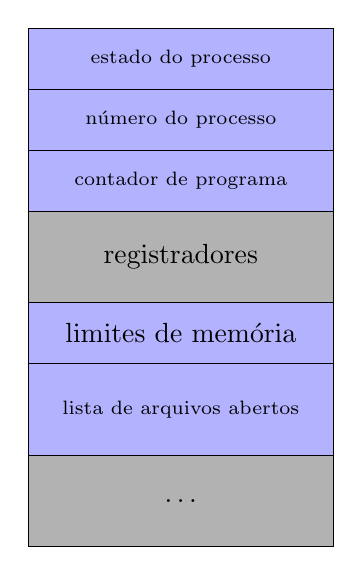
\begin{tikzpicture}[every rectangle/.style={minimum width=\recbase},
    scale=0.775,mem/.style={fill=gray!60},
    var/.style={fill=blue!30}]
    
    \draw[var] (0,2+5.5*\recheight) rectangle (\recbase,2+6.5*\recheight)
    node[midway] {\scriptsize{estado do processo}};
    \draw[var] (0,2+4.5*\recheight) rectangle (\recbase,2+5.5*\recheight)
    node[midway] {\scriptsize{número do processo}};
    \draw[var] (0,2+3.5*\recheight) rectangle (\recbase,2+4.5*\recheight)
    node[midway] {\scriptsize{contador de programa}};
    \draw[mem] (0,2+2*\recheight) rectangle (\recbase,2+3.5*\recheight) node[midway] {registradores};
    \draw[var] (0,2+\recheight) rectangle (\recbase,2+2*\recheight) node[midway] {limites de
    memória};
    \draw[var] (0,1.5) rectangle (\recbase,2+\recheight) node[midway] {\scriptsize{lista de
    arquivos abertos}};
    \draw[mem] (0,0) rectangle (\recbase,1.5*\recheight) node[midway] {$\ldots$};
  \end{tikzpicture}
\end{center}

\caption{Bloco de controle do processo.}
\label{proc:fig:pcb}

\end{figure}

\end{center}
\end{column}
} 
\end{columns}
\end{frame}

\subsection{Estados dos processos}

\begin{frame}{Estados de um processo}
  
\begin{block}{Estados}
  \begin{description}
  \item[Novo] O processo está sendo criado.
  \item[Executando] As instruções estão sendo executadas.
  \item[Esperando] O processo está esperando pela ocorrência de algum
    evento (como um término de E/S ou um sinal).
  \item[Pronto] O processo está esperando para ser designado a um processador.
  \item[Terminado] O processo terminou sua execução.
  \end{description}
\end{block}

\end{frame}

\begin{frame}[fragile]{Transição dos estados de um processo}
  
	\makeatletter
\colorlet{new}{white}
\colorlet{ready}{blue}
\colorlet{exec}{red}
\colorlet{wait}{orange!70!black}
\colorlet{end}{black}

  \begin{center}
    \begin{tikzpicture}[every node/.style={font=\scriptsize},
      state/.style={ellipse,font=\bf,draw},
      transition/.style={->,>=latex},
      statelabel/.style={midway,font=\bf\tiny,text width=1.5cm,align=center}]
      \def\@@ds{1.75cm}
      \node[fill=new,draw] (new) at (0,0) {\bf\large novo};
      \node[above of=new,yshift=-.5cm] {\footnotesize\tt cria PCB};
      \node[color=white,state,fill=ready] (ready) at (2*\@@ds,-\@@ds) {pronto};
      \node[color=yellow,state,fill=exec] (exec) at (4*\@@ds,0) {executando};
      \node[color=gray!30,state,fill=wait] (wait) at (2*\@@ds,\@@ds) {esperando};
      \node[white,fill=black] (end) at (4.5*\@@ds,\@@ds) {t\'ermino};
      \node[above of=end,yshift=-.35cm] {\footnotesize\tt apaga PCB};
    
      \draw[transition,draw=ready] (new) .. controls +(down:8mm) and +(left:32mm) .. (ready)  node[statelabel,left] {enviado para a fila};
      \draw[transition,draw=exec] (ready) .. controls +(right:32mm) and +(down:8mm) .. (exec)  node[statelabel,right] {escalonado para execu\c{c}\~ao};
      \draw[transition,draw=ready] (exec.west) .. controls +(left:8mm) and +(up:8mm) .. (ready.north)  node[statelabel,above] {escalonado para a fila};
      \draw[transition,draw=wait] (exec.north) .. controls +(up:16mm) and +(right:4mm) .. (wait.east) node[statelabel,above] {requisi\c{c}\~ao E/S};
      \draw[transition,draw=ready] (wait.west) .. controls +(left:16mm) and +(left:16mm) .. (ready.west) node[statelabel,right] {t\'ermino E/S};
      \draw[transition,draw=end] (exec) .. controls +(right:32mm) and +(right:24mm) .. (end) node[statelabel,left] {t\'ermino do processo};
      
    \end{tikzpicture}

  \end{center}
  \makeatother

\end{frame}

\begin{frame}{Sequência dos PCBs}{Transição de estados}

\begin{center}
	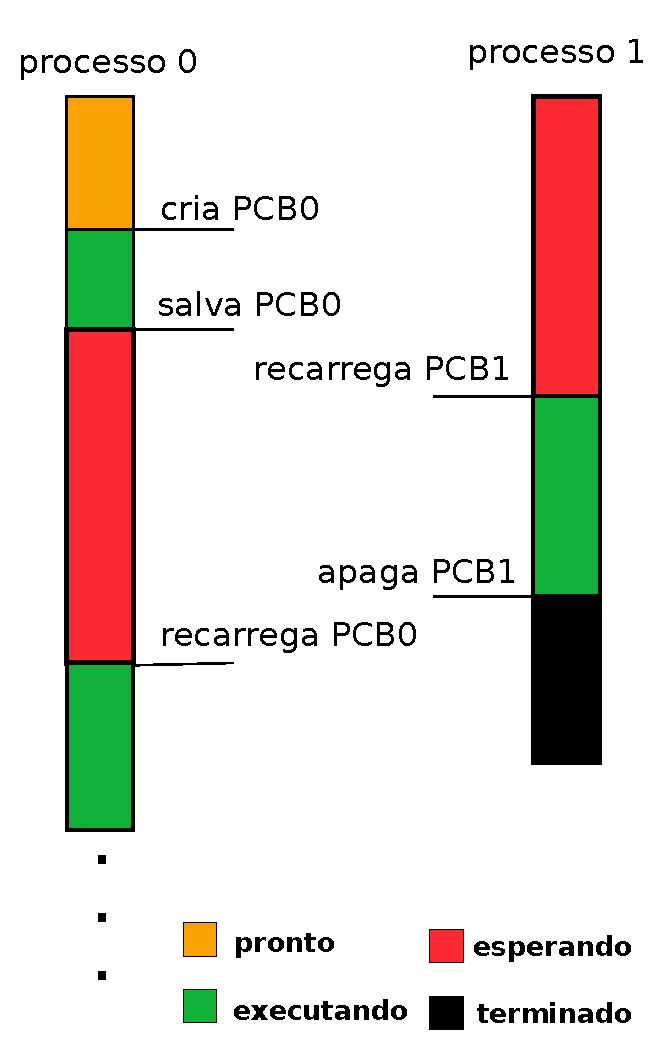
\includegraphics[scale=0.45]{pcb-sequence}
\end{center}
\end{frame}

\subsection{Criação de um processo}

% A criação de processos em sistemas derivados do Unix usa a função
% \lstinline{fork()}, que geralmente segue as seguintes etapas:

% \begin{enumerate}
% \item Cria a tabela de dados do processo;
% \item Checa os limites do processo;
% \item Inicializa a tabela de dados;
% \item Atribui um número de identificação do processo;
% % Duplica (Processo -> COW), compartilha (Threads)
% \item ``Duplica'' ou compartilha:
%   \begin{itemize}
%   \item Arquivos abertos;
%   \item Sistema de arquivos;
%   \item Espaço de endereçamento (memória);
%   \item Sinais.
%   \end{itemize}
% \end{enumerate}
\lstset{emph={%  
    fork, wait, exit%
    },emphstyle={\color{red}\bfseries\underbar}%
}%
\begin{frame}[fragile]
  \frametitle{Criação de um processo}
  \framesubtitle{Derivados do Unix: \lstinline{fork()}}
  \begin{columns}
    \begin{column}{.6\textwidth}\scriptsize
\begin{lstlisting}
int pid = fork();
if(pid > 0){
    printf("proc-pai: filho=%d\n", pid);
    pid = wait((int *) 0);
    printf("proc-filho %d terminou\n", pid);
} else if(pid == 0){
    printf("proc-filho: saindo\n");
    exit(0);
} else {
    printf("erro\n");
}
      \end{lstlisting}
    \end{column}
    \begin{column}{.4\textwidth}
      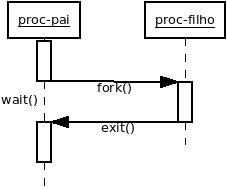
\includegraphics[scale=.525]{fork.png}
    \end{column}
  \end{columns}
\end{frame}

%%%%%%%%%%%%%%%%%%%%%%%%%%%%%%%%%%%%%%%%%%%%%%%%%%%%%%%%%%%%%%%%
%% BUFFER
%%%%%%%%%%%%%%%%%%%%%%%%%%%%%%%%%%%%%%%%%%%%%%%%%%%%%%%%%%%%%%%%

\ifnum1=2
\begin{frame}{Exemplos e aplicações}

  \begin{itemize}
    \item \href{http://lxr.linux.no/\#linux+v2.6.37.1/include/linux/sched.h\#L1182}{Analisar os membros da estrutura de {\tt task\_struct}}
  \item Monitoramento de processos usando as ferramentas do Linux {\tt
      ps}, {\tt top}, {\tt atop}, {\tt htop}.
  \item \href{http://adrianoholanda.org/edu/file.php/3/codigo_fonte/proc_cria_posix.c}{Criação
      de processos utilizando a API Posix.}
  \item \href{http://adrianoholanda.org/edu/file.php/3/codigo_fonte/proc_cria_win32.c}{Criação
      de processos usando chamadas de sistema do Windows.}
  \end{itemize}
  
\end{frame}
\fi
